%% =====================================================================
%%  X-UAD  (revision 5)
%%  IEEE conference format (IEEEtran).  Compile with pdflatex + bibtex:
%%     pdflatex xuad_v2 && bibtex xuad_v2 && pdflatex xuad_v2 && pdflatex xuad_v2
%%  Every number in the tables is \input from tables/.
%% =====================================================================
\documentclass[conference]{IEEEtran}
\IEEEoverridecommandlockouts

\usepackage{iftex}
% XeTeX has no Type-1 Times, so bold and italic would silently disappear.
% Use the Times clone TeX Gyre Termes there. pdflatex keeps IEEEtran's own Times.
\ifXeTeX
  \usepackage{fontspec}
  \setmainfont{texgyretermes}[Extension=.otf, UprightFont=*-regular,
    BoldFont=*-bold, ItalicFont=*-italic, BoldItalicFont=*-bolditalic]
\fi
\usepackage{cite}
\usepackage{amsmath,amssymb,amsfonts}
\usepackage{graphicx}
\usepackage{booktabs}
\usepackage{multirow}
\usepackage{flafter} % floats never appear before their first mention, keeping citation order
\usepackage{adjustbox}
\usepackage{tikz} % Fig. 1 is drawn in TikZ (figures/architecture_tikz.tex)
\usetikzlibrary{positioning,arrows.meta,calc,fit,backgrounds}
\usepackage{placeins} % \FloatBarrier before the Conclusion keeps every table and figure above the back matter
\usepackage{xcolor}
\usepackage{textcomp}
\usepackage{url}
\usepackage[hidelinks]{hyperref}

\newcommand{\bs}[1]{\boldsymbol{#1}}
\newcommand{\R}{\mathbb{R}}
\newcommand{\ket}[1]{\lvert #1 \rangle}
\newcommand{\bra}[1]{\langle #1 \rvert}
\newcommand{\braket}[2]{\langle #1 \vert #2 \rangle}
% bold subsection headings so that every topic is clearly visible
\newcommand{\sub}[1]{\subsection{\texorpdfstring{\textbf{#1}}{#1}}}

\newlength{\colw}
% single-column float width. In the one-column copy small tables and figures are capped
\makeatletter
\AtBeginDocument{\if@twocolumn\setlength{\colw}{\columnwidth}\else\setlength{\colw}{0.62\textwidth}\fi}
% table width cap: the column in two-column mode, the full text width in the one-column copy
\newlength{\tabw}
\AtBeginDocument{\if@twocolumn\setlength{\tabw}{\columnwidth}\else\setlength{\tabw}{\textwidth}\fi}
\newcommand{\fittab}[1]{\begin{adjustbox}{max width=\tabw}#1\end{adjustbox}}
% float placement: top of column in the IEEE two-column layout; in the one-column copy
% floats may sit where they are mentioned, which avoids half-empty pages
\AtBeginDocument{\if@twocolumn\def\fps@table{t}\def\fps@figure{t}%
  \else\def\fps@table{!htbp}\def\fps@figure{!htbp}\fi}
\renewcommand{\topfraction}{0.85}
\renewcommand{\textfraction}{0.10}
\renewcommand{\floatpagefraction}{0.75}
\renewcommand{\dbltopfraction}{0.85}
\renewcommand{\dblfloatpagefraction}{0.75}
% start a new, centred row of author blocks
\newcommand{\linebreakand}{\end{@IEEEauthorhalign}\hfill\mbox{}\par\mbox{}\hfill\begin{@IEEEauthorhalign}}
\makeatother

\begin{document}

\title{X-UAD\,---\,An Uncertainty-Aware and Self-Explaining Detector for
Physical and Digital Face Attacks}

\author{%
\IEEEauthorblockN{Amrutha Babu}
\IEEEauthorblockA{\textit{School of Computer Science}\\
\textit{and Engineering}\\
\textit{Vellore Institute of Technology}\\
Vellore, India\\
amrutha.babu2024@vitstudent.ac.in}
\and
\IEEEauthorblockN{Swethaa Premnath}
\IEEEauthorblockA{\textit{School of Computer Science}\\
\textit{and Engineering}\\
\textit{Vellore Institute of Technology}\\
Vellore, India\\
swethaa.premnath2024@vitstudent.ac.in}
\and
\IEEEauthorblockN{Vividha Senthil Mohan}
\IEEEauthorblockA{\textit{School of Computer Science}\\
\textit{and Engineering}\\
\textit{Vellore Institute of Technology}\\
Vellore, India\\
vividha.senthil2024@vitstudent.ac.in}
\linebreakand
\IEEEauthorblockN{Muthunagai S U$^{*}$}
\IEEEauthorblockA{\textit{School of Computer Science}\\
\textit{and Engineering}\\
\textit{Vellore Institute of Technology}\\
Vellore, India\\
muthunagai.su@vit.ac.in\\
$^{*}$Corresponding author}
\and
\IEEEauthorblockN{Nivedha K}
\IEEEauthorblockA{\textit{School of Computer Science}\\
\textit{and Engineering}\\
\textit{Vellore Institute of Technology}\\
Vellore, India\\
nivitha.k@vit.ac.in}
}

\maketitle

\begin{abstract}
Face recognition systems can be fooled in two ways. Physical attacks show the camera
a printed photo, a replayed video or a mask, while digital attacks change the
captured image through face swapping, expression transfer, fully synthetic faces or
adversarial noise. Most detectors handle only one of these groups. They also give a
single score without saying how sure they are, where the fake evidence lies or why
the decision was made. The aim of this work is a single detector that handles both
groups and explains its own decisions. The proposed model, X-UAD, joins a central
difference convolution stem and a frequency branch with a transformer that uses
Adaptive Quantum Attention, which compares image patches through squared overlaps
that suit repeating patterns such as screen stripes and printer dots. An evidential
output layer gives an uncertainty score that is trained on blends of two attack
types. A decoder marks the attack region and a rule-based module writes an
explanation using only the measured values. On a simulated benchmark of eight attack
types X-UAD reaches 0.42\% ACER on seen attacks and 80.1\% region-level IoU for
localisation. It also gives the highest detection rate on unseen attack types at
77.5\%. All tested methods still fail when the camera domain changes.
\end{abstract}

\begin{IEEEkeywords}
face anti-spoofing, presentation attack detection, deepfake detection, unified
attack detection, vision transformer, quantum-inspired attention, evidential deep
learning, uncertainty estimation, open-set recognition, explainable AI
\end{IEEEkeywords}

% =====================================================================
\section{Introduction}
% =====================================================================
Face unlock and face verification systems can be attacked in front of the camera.
A printed photo of the owner, a video replayed on a phone screen or a silicone mask
can all be shown to the sensor. These are \emph{physical} attacks. Each one leaves
a physical trace behind, such as the dot pattern of a printer, the pixel grid of a
screen that turns into a moir\'e pattern or the smooth waxy surface of silicone.

A face image can also be changed \emph{after} a real photo has been taken. The
identity can be swapped, the expression can be copied from another person, a face
that never existed can be generated or a small pattern of noise can be added that
flips the decision of a classifier. These are \emph{digital} attacks. Their traces
look very different, for example blending edges around a swapped face, mismatched
resolution, checkerboard patterns from the upsampling layers of a generator and
unusual peaks in the frequency spectrum.

Because the two kinds of traces look so different, the two research areas grew up
separately. Face anti-spoofing focused on texture and depth cues
\cite{liu2018auxiliary,yu2020cdcn,yu2021revisiting,wang2022ssan}, while face forgery
detection focused on frequency and blending cues
\cite{rossler2019ff,li2020celebdf,frank2020frequency,wang2020cnnspot}. A real system
needs one decision, one threshold and one record of why the decision was taken.
Recent work
\cite{yu2024unified,yuan2024challenge,ma2025uniattackplus,chen2025uniattack,zhang2024unidefense}
built joint datasets and joint detectors for both groups. On attack types seen during
training these detectors reach an ACER of about $0.5$ to $1.4\%$. When one attack
family is held out during training the error rises to between $22$ and $44\%$ with
large variation between runs \cite{yu2024unified}. Joint detection is therefore close
to solved for known attacks but remains open for new ones.

Three more abilities are missing from most of this work. The first is a real sense of
\emph{not knowing}. A softmax output must spread all of its probability over the known
classes, so a completely new attack is still given high confidence for whichever
known class it looks most like. A second-order belief is needed that can stay close
to empty when the input looks like nothing learned before. The second is \emph{evidence
localisation}. Depth-map supervision \cite{liu2018auxiliary,yu2021revisiting} works
for physical attacks because a photo or a screen is flatter than a real face. Depth
says nothing about a swapped face that came from a live three-dimensional capture.
The third is an \emph{explanation tied to the decision}. Recent methods pass the face
image to a multimodal language model and ask it to describe what looks fake
\cite{huang2024ffaa,guo2025m2f2det}. The language model never sees the internal state
of the detector, so its text can mention artifacts such as a screen bezel that are
not in the frame or were never used by the detector.

This paper presents X-UAD, a single model that detects physical and digital face
attacks together, reports how uncertain it is, marks where the evidence lies and
explains its decision with text built only from its own measured values. Three ideas
make this possible. \textbf{Adaptive Quantum Attention (AQA)} adds a second scoring
channel to normal attention. Much of the evidence for face attacks, such as a moir\'e
beat, a checkerboard or a spectral peak, appears in the \emph{squared size} of a
projection and its sign carries no meaning. The new channel compares two tokens by the
squared overlap of their unit vectors after a learnable rotation, which follows the
Born rule of quantum measurement. A learned gate mixes this channel with the normal
dot product. The rotations need only $\mathcal{O}(dL)$ angles instead of the
$\mathcal{O}(d^{2})$ weights of a linear layer. A \textbf{quantum evidence basis}, which
is a set of orthonormal vectors built by the same kind of rotation, is measured
against every spatial token. The resulting probabilities are used as classification
features and are also shown unchanged as the explanation. \textbf{Pseudo-Unseen
Evidence Suppression (PUES)} blends two training images from different attack
families. No real camera or generator can produce such a blend, so it acts as a free
stand-in for a new attack. The model is trained to give low evidence on these blends,
which teaches the uncertainty output how an unknown input should look.

Every forward pass also writes a typed numeric \textbf{evidence record}. The text
explanation is produced only from this record by a rule-based generator in which every
sentence is guarded by a numeric condition, so the generator cannot invent facts.
Since no capture-based dataset marks \emph{where} the attack evidence lies, a
difficulty-calibrated, identity-disjoint benchmark of eight attack families with
pixel-level evidence masks was also built, together with seen-attack,
leave-one-attack-out and cross-domain test protocols.

Section~\ref{sec:related} reviews related work. Section~\ref{sec:method} describes the
proposed work including the benchmark and the model. Section~\ref{sec:exp} reports the
results and Section~\ref{sec:concl} concludes the paper.

% =====================================================================
\section{Related Work}\label{sec:related}
% =====================================================================

\sub{Physical Presentation Attack Detection}
Early face anti-spoofing treated liveness as a texture classification problem.
Auxiliary supervision \cite{liu2018auxiliary} replaced the plain real or fake label
with a pseudo-depth map and an rPPG signal as extra training targets. Central
Difference Convolution \cite{yu2020cdcn} changed the first layers of the network so
that they respond to fine texture that does not depend on lighting. It is still one of
the strongest light backbones for physical attacks. Pixel-wise supervision was studied
further in \cite{yu2021revisiting}. Later work tried to generalise across cameras and
lighting through adversarial domain generalisation \cite{shao2019mada}, single-side
domain generalisation \cite{jia2020ssdg} and style-shuffled feature separation
\cite{wang2022ssan}. All of these methods assume that the attack happens in front of
the camera. None of them can handle a real capture that was edited afterwards.

\sub{Digital Forgery Detection}
FaceForensics++ \cite{rossler2019ff} and Celeb-DF \cite{li2020celebdf} are the main
benchmarks of this area. The cue that transfers best is spectral. Generators leave
periodic artifacts from their upsampling layers \cite{odena2016checkerboard}, which
show up as peaks in the Fourier magnitude \cite{frank2020frequency}. This is a large
part of why simple detectors transfer well across generator types
\cite{wang2020cnnspot}. These detectors have no idea of a re-capture medium and fail
on printed or replayed attacks.

\sub{Unified Physical and Digital Detection}
UniAttackData \cite{yu2024unified} is an identity-consistent dataset in which the same
person appears both as genuine and under every attack type, so identity cannot become
a shortcut. It comes with a vision-language detector trained with teacher-student
prompts. The CVPR 2024 and ICCV 2025 challenges built on it
\cite{yuan2024challenge,ma2025uniattackplus} with nearly $2{,}900$ subjects and $54$
attack types. Methods built on large pretrained multimodal backbones led the
leaderboard while single-modality CNNs stayed above $20\%$ ACER on the harder
protocol. UniDefense \cite{zhang2024unidefense} uses dual-space reconstruction for the
same goal. None of these systems gives an uncertainty output, an evidence map or a
real explanation.

\sub{Uncertainty and Open-Set Recognition}
Maximum softmax probability \cite{hendrycks2017msp} is a weak signal for unknown inputs
because softmax is closed-set. Prior networks \cite{malinin2018prior} and evidential
deep learning \cite{sensoy2018edl}, based on subjective logic
\cite{josang2016subjective}, place a Dirichlet distribution over the class simplex so
that total evidence and vacuity become outputs of the model. Outlier exposure
\cite{hendrycks2019oe} showed that even a rough stand-in for unknown inputs during
training helps more than any purely internal uncertainty score. Open-set
single-domain generalisation was recently studied for anti-spoofing alone
\cite{liu2024openset}. Evidential uncertainty has not yet been joined with unified
physical and digital detection and no earlier method builds its outlier stand-in from
the attack taxonomy itself.

\sub{Explainability and Language-Model Forensics}
Attention rollout \cite{abnar2020rollout} and deletion and insertion tests
\cite{petsiuk2018rise} are the usual tools for checking whether an explanation
reflects the decision of a model. FFAA \cite{huang2024ffaa} fine-tunes a multimodal
LLM for open-world forgery analysis and M2F2-Det \cite{guo2025m2f2det} joins CLIP with
an LLM for interpretable forged-face detection. Both produce fluent text after the
fact. The language model sees the image but not the internal evidence of the
detector, so its account cannot be checked against the decision.

\sub{Quantum-Inspired Attention}
Quantum vision transformers \cite{cherrat2024qvt} and quantum self-attention
\cite{comajoan2024qgluon,evans2025on} replace linear projections with parameterised
quantum circuits and report accuracy close to classical vision transformers with far
fewer parameters. Quantum adaptive self-attention \cite{chen2025qasa} places such a
circuit inside one encoder layer and compares it with classical controls of equal
size. This line of work is driven by parameter savings on generic image
classification. It has not been applied to a task whose evidence is an interference
pattern and it offers no explanation.

Each of these lines covers only part of what a deployed system needs, as summarised in
Table~\ref{tab:prior}, where \emph{partial} means that the ability exists only for one
attack group or only as a proxy. The missing parts also depend on each other.
Covering more attack families makes uncertainty more important. Uncertainty makes
explanation more important, since a reviewer who is handed an uncertain sample needs
to know what the model saw. An explanation is only worth trusting when it comes from
the same internal evidence that produced the decision.

\begin{table*}
\centering
\caption{Comparison with prior work}
\label{tab:prior}
\scriptsize
\setlength{\tabcolsep}{4pt}
\resizebox{0.9\textwidth}{!}{%
\begin{tabular}{lccccccc}
\toprule
 & Physical & Digital & Second-order & Explicit & Evidence & Text & Explanation bound \\
Representative work & attacks & attacks & uncertainty & unknown class & localisation & explanation & to the decision \\
\midrule
CDCN++ \cite{yu2020cdcn}, pixel-wise FAS \cite{yu2021revisiting} & yes & no & no & no & partial (depth proxy) & no & --- \\
SSAN \cite{wang2022ssan}, SSDG \cite{jia2020ssdg} & yes & no & no & no & no & no & --- \\
Frequency forensics \cite{frank2020frequency,wang2020cnnspot} & no & yes & no & no & no & no & --- \\
UniAttackDetection \cite{yu2024unified}, UniDefense \cite{zhang2024unidefense} & yes & yes & no & no & no & no & --- \\
Challenge winners \cite{ma2025uniattackplus} & yes & yes & no & no & no & no & --- \\
Evidential and open-set \cite{sensoy2018edl,liu2024openset} & partial & no & yes & yes & no & no & --- \\
FFAA \cite{huang2024ffaa}, M2F2-Det \cite{guo2025m2f2det} & no & yes & no & partial & partial & yes & no (post-hoc) \\
Quantum ViT \cite{cherrat2024qvt,evans2025on,chen2025qasa} & no & no & no & no & no & no & --- \\
\midrule
\textbf{X-UAD (proposed)} & \textbf{yes} & \textbf{yes} & \textbf{yes} & \textbf{yes} & \textbf{yes} & \textbf{yes} & \textbf{yes} \\
\bottomrule
\end{tabular}}
\end{table*}

% =====================================================================
\section{Proposed Work}\label{sec:method}
% =====================================================================

\sub{Overview}
X-UAD maps a face crop $\bs{x}\in\R^{3\times H\times W}$ to six outputs,
\begin{equation}
\bs{x}\;\longmapsto\;\bigl(\bs{\alpha},\;u,\;\bs{M},\;\bs{\Pi},\;r,\;\tau\bigr),
\label{eq:map}
\end{equation}
where in Eq.~\eqref{eq:map} $\bs{\alpha}\in\R^{K}_{>0}$ are Dirichlet concentrations over
the $K=8$ classes, $u\in[0,1]$ is the vacuity, a single number that grows when the
model has little evidence, $\bs{M}$ is the spoof-evidence map, $\bs{\Pi}$ is the
quantum evidence spectrum over tokens and basis modes, $r$ is the risk score and
$\tau$ is the text explanation. All six come from one forward pass
(Fig.~\ref{fig:arch}). A central-difference stem and a spectral branch produce tokens,
which are processed by a stack of AQA blocks. The quantum evidence basis is measured
against the output tokens. An evidential head, a localisation decoder and a risk
calibrator read out the results, after which the reasoning module turns the record
into text. Table~\ref{tab:notation} lists the main symbols and abbreviations.

\begin{figure*}
\centering
\resizebox{\textwidth}{!}{% X-UAD architecture, drawn in TikZ so it stays vector and uses the paper's fonts.
% \input inside a figure; needs amsmath, \usepackage{tikz} and
% \usetikzlibrary{positioning,arrows.meta,calc,fit,backgrounds}.
\providecommand{\ArchTtl}{\footnotesize\bfseries}
\providecommand{\ArchLbl}{\bfseries}
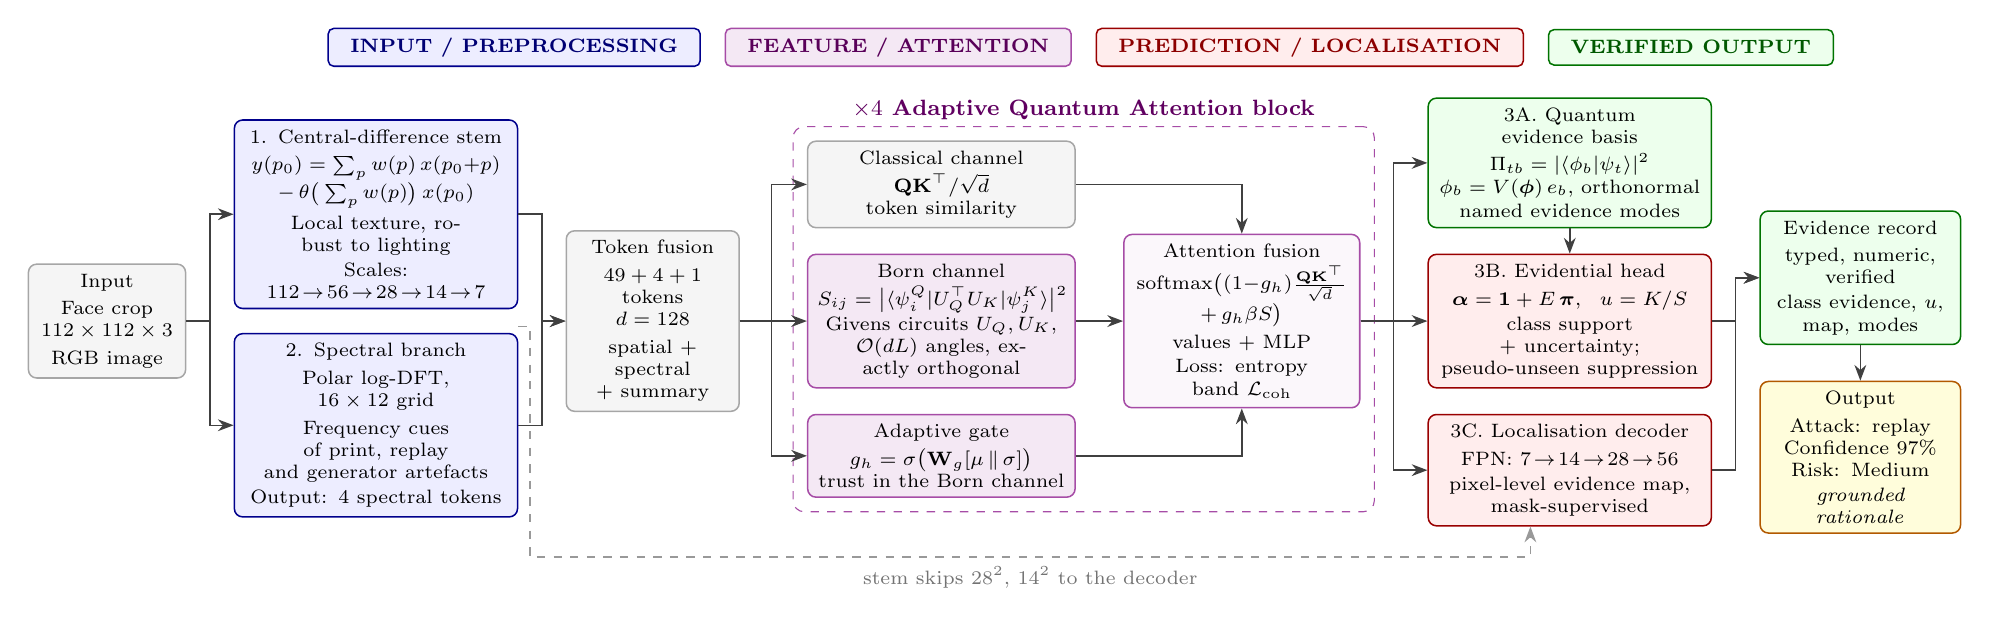
\begin{tikzpicture}[
  font=\scriptsize, >={Stealth[length=2mm]}, line width=0.55pt,
  node distance=0.32cm and 0.55cm,
  box/.style={draw, rounded corners=3pt, align=center, inner sep=3.5pt, text width=#1},
  inbox/.style={box=#1, draw=gray!70, fill=gray!8},
  bluebox/.style={box=#1, draw=blue!55!black, fill=blue!7},
  purbox/.style={box=#1, draw=violet!70, fill=violet!9},
  fusbox/.style={box=#1, draw=violet!70, fill=violet!3},
  redbox/.style={box=#1, draw=red!60!black, fill=red!7},
  grnbox/.style={box=#1, draw=green!45!black, fill=green!7},
  outbox/.style={box=#1, draw=orange!70!black, fill=yellow!14},
  legend/.style={draw, rounded corners=2pt, minimum height=0.45cm, inner xsep=8pt,
                 font=\scriptsize\bfseries},
  flow/.style={->, draw=black!75},
  skip/.style={->, draw=black!40, dashed},
]

% ---------------- left: input, stem, spectral, tokens ----------------
\node[inbox=1.75cm] (in) {%
  {\ArchTtl Input}\\[2pt] Face crop\\ \mbox{$112\times112\times3$}\\[2pt] RGB image};

\node[bluebox=3.35cm, above right=0.15cm and 0.6cm of in.east, anchor=south west] (stem) {%
  {\ArchTtl 1. Central-difference stem}\\[2pt]
  \mbox{$y(p_0)=\sum_{p} w(p)\,x(p_0{+}p)$}\\ \mbox{$-\,\theta\big(\sum_{p} w(p)\big)\,x(p_0)$}\\[2pt]
  Local texture, robust to lighting\\[1pt]
  {\ArchLbl Scales:} \mbox{$112\!\to\!56\!\to\!28\!\to\!14\!\to\!7$}};

\node[bluebox=3.35cm, below right=0.15cm and 0.6cm of in.east, anchor=north west] (spec) {%
  {\ArchTtl 2. Spectral branch}\\[2pt]
  Polar log-DFT, \mbox{$16\times12$} grid\\[2pt]
  Frequency cues of print, replay\\ and generator artefacts\\[1pt]
  {\ArchLbl Output:} 4 spectral tokens};

\node[inbox=1.95cm, anchor=west] (tok) at ($(stem.east |- in.east)+(0.6,0)$) {%
  {\ArchTtl Token fusion}\\[2pt]
  \mbox{$49+4+1$} tokens\\ \mbox{$d=128$}\\[2pt]
  spatial + spectral\\ + summary};

% ---------------- AQA block ----------------
\node[purbox=3.15cm, right=0.85cm of tok] (born) {%
  {\ArchTtl Born channel}\\[2pt]
  \mbox{$S_{ij}=\big|\langle\psi^{Q}_i|U_Q^{\top}U_K|\psi^{K}_j\rangle\big|^2$}\\[1pt]
  Givens circuits \mbox{$U_Q,U_K$},\\ \mbox{$\mathcal{O}(dL)$} angles, exactly orthogonal};

\node[inbox=3.15cm, above=of born] (cls) {%
  {\ArchTtl Classical channel}\\[2pt] \mbox{$\mathbf{Q}\mathbf{K}^{\top}/\sqrt{d}$}\\ token similarity};

\node[purbox=3.15cm, below=of born] (gate) {%
  {\ArchTtl Adaptive gate}\\[2pt] \mbox{$g_h=\sigma\big(\mathbf{W}_g[\mu\,\|\,\sigma]\big)$}\\
  trust in the Born channel};

\node[fusbox=2.75cm, right=0.6cm of born] (fus) {%
  {\ArchTtl Attention fusion}\\[2pt]
  \mbox{$\mathrm{softmax}\big((1{-}g_h)\tfrac{\mathbf{QK}^{\top}}{\sqrt d}$}\\ \mbox{$+\,g_h\beta S\big)$}\\[2pt]
  values + MLP\\[1pt]
  {\ArchLbl Loss:} entropy band \mbox{$\mathcal{L}_{\mathrm{coh}}$}};

\begin{scope}[on background layer]
  \node[draw=violet!70, dashed, rounded corners=4pt, inner sep=5pt,
        fit=(cls)(born)(gate)(fus)] (aqa) {};
\end{scope}
\node[font=\footnotesize\bfseries, text=violet!75!black, anchor=south, inner sep=2pt]
  at (aqa.north) {\mbox{$\times4$} Adaptive Quantum Attention block};

% ---------------- heads ----------------
\node[redbox=3.35cm, right=0.85cm of fus] (evi) {%
  {\ArchTtl 3B. Evidential head}\\[2pt]
  \mbox{$\boldsymbol{\alpha}=\mathbf{1}+E\,\boldsymbol{\pi},\ \ u=K/S$}\\[1pt]
  class support + uncertainty;\\ pseudo-unseen suppression};

\node[grnbox=3.35cm, above=of evi] (basis) {%
  {\ArchTtl 3A. Quantum evidence basis}\\[2pt]
  \mbox{$\Pi_{tb}=|\langle\phi_b|\psi_t\rangle|^2$}\\ \mbox{$\phi_b=V(\boldsymbol{\phi})\,e_b$}, orthonormal\\[1pt]
  named evidence modes};

\node[redbox=3.35cm, below=of evi] (loc) {%
  {\ArchTtl 3C. Localisation decoder}\\[2pt]
  FPN: \mbox{$7\!\to\!14\!\to\!28\!\to\!56$}\\[1pt]
  pixel-level evidence map,\\ mask-supervised};

% ---------------- verified output ----------------
\node[grnbox=2.3cm, right=0.6cm of evi, yshift=0.55cm] (rec) {%
  {\ArchTtl Evidence record}\\[2pt]
  typed, numeric,\\ verified\\[1pt]
  class evidence, \mbox{$u$},\\ map, modes};

\node[outbox=2.3cm, below=0.45cm of rec] (out) {%
  {\ArchTtl Output}\\[2pt]
  Attack: replay\\ Confidence 97\%\\ Risk: Medium\\[1pt]
  \textit{grounded rationale}};

% ---------------- legend (above, centred on the diagram) ----------------
\coordinate (top) at ($(aqa.north)+(0,0.75)$);
\node[legend, draw=violet!70, fill=violet!9, text=violet!70!black, anchor=south east]
  (L2) at ($(top -| aqa.center)+(-0.15,0)$) {FEATURE / ATTENTION};
\node[legend, draw=blue!55!black, fill=blue!7, text=blue!45!black, left=0.3cm of L2] (L1) {INPUT / PREPROCESSING};
\node[legend, draw=red!60!black, fill=red!7, text=red!55!black, right=0.3cm of L2] (L3) {PREDICTION / LOCALISATION};
\node[legend, draw=green!45!black, fill=green!7, text=green!35!black, right=0.3cm of L3] (L4) {VERIFIED OUTPUT};

% ---------------- arrows ----------------
\draw[flow] (in.east) -- ++(0.3,0) |- (stem.west);
\draw[flow] (in.east) -- ++(0.3,0) |- (spec.west);
\draw[flow] (stem.east) -- ++(0.3,0) |- (tok.west);
\draw[flow] (spec.east) -- ++(0.3,0) |- (tok.west);
\draw[flow] (tok.east) -- (born.west);
\draw[flow] (tok.east) -- ++(0.4,0) |- (cls.west);
\draw[flow] (tok.east) -- ++(0.4,0) |- (gate.west);
\draw[flow] (cls.east) -| (fus.north);
\draw[flow] (born.east) -- (fus.west);
\draw[flow] (gate.east) -| (fus.south);
\draw[flow] (fus.east) -- ++(0.42,0) |- (basis.west);
\draw[flow] (fus.east) -- (evi.west);
\draw[flow] (fus.east) -- ++(0.42,0) |- (loc.west);
\draw[flow] (basis.south) -- (evi.north);
\draw[flow] (evi.east) -- ++(0.3,0) |- (rec.west);
\draw[flow] (loc.east) -- ++(0.3,0) |- (rec.west);
\draw[flow] (rec.south) -- (out.north);
\coordinate (skipy) at ($(gate.south)+(0,-0.75)$);
\draw[skip] (stem.east |- spec.north) ++(0,0.08) -- ++(0.15,0) coordinate (s1)
  -- (s1 |- skipy) -- ($(loc.south |- skipy)+(-0.5,0)$)
  node[pos=0.5, below, text=black!55] {stem skips \mbox{$28^2$}, \mbox{$14^2$} to the decoder}
  -- ($(loc.south)+(-0.5,0)$);
\end{tikzpicture}
}
\caption{Architecture of X-UAD}
\label{fig:arch}
\end{figure*}

In Fig.~\ref{fig:arch} the stem supplies fine texture evidence that does not depend on
lighting and the spectral branch supplies periodic evidence that cannot be seen at the
token resolution. Each AQA block scores token pairs with a gated mix of the classical
dot product and the Born-rule overlap between rotated unit vectors. The Born
probabilities of the evidence basis feed the classifier \emph{and} are exported
unchanged as the explanation. This is what ties the explanation to the decision.

\begin{table*}
\centering
\caption{Notation and abbreviations}
\label{tab:notation}
\scriptsize
\setlength{\tabcolsep}{3pt}
\begin{minipage}[t]{0.49\textwidth}
\centering
\begin{tabular}[t]{@{}p{0.25\linewidth}p{0.72\linewidth}@{}}
\toprule
Symbol & Meaning \\
\midrule
$\bs{x}$, $K$, $s$ & Input face crop, number of classes, attack strength \\
$\bs{\alpha}$, $u$ & Dirichlet concentrations, vacuity $u=K/S$ \\
$\bs{M}$, $\bs{\Pi}$ & Evidence map, quantum evidence spectrum \\
$r$, $\tau$ & Risk score, text explanation \\
$d$, $L$ & Head dimension, depth of a rotation circuit \\
$G(\vartheta)$, $U$ & Givens rotation, rotation circuit \\
$S_{ij}$ & Born-rule overlap of tokens $i$ and $j$ \\
$g_{h}$, $\beta$ & Gate of head $h$, Born-channel temperature \\
$\bs{A}$, $\mathcal{H}$ & Attention matrix, its mean row entropy \\
$\ket{\phi_{b}}$, $B$ & Evidence basis vector, number of modes \\
$\bs{\pi}$, $E$, $S$ & Class direction, total evidence, $S=K+E$ \\
$\hat{p}_{k}$ & Projected probability of class $k$ \\
$\tilde{\bs{x}}$, $\rho$ & PUES blend, PUES target ratio \\
$\varsigma_{k}$, $a$ & Severity of family $k$, evidence area \\
$\mathcal{L}$, $w$ & Loss terms, loss weights \\
\bottomrule
\end{tabular}
\end{minipage}\hfill
\begin{minipage}[t]{0.49\textwidth}
\centering
\begin{tabular}[t]{@{}p{0.20\linewidth}p{0.77\linewidth}@{}}
\toprule
Abbreviation & Full form \\
\midrule
X-UAD & Explainable Unified Attack Detection \\
AQA & Adaptive Quantum Attention \\
PUES & Pseudo-Unseen Evidence Suppression \\
CDC & Central Difference Convolution \\
APCER & Attack Presentation Classification Error Rate \\
BPCER & Bona fide Presentation Classification Error Rate \\
ACER & Average Classification Error Rate \\
AUC & Area Under the Curve \\
AUROC & Area Under the Receiver Operating Characteristic curve \\
EER & Equal Error Rate \\
ECE & Expected Calibration Error \\
IoU & Intersection over Union \\
PGD & Projected Gradient Descent \\
LFW & Labeled Faces in the Wild \\
MLLM & Multimodal Large Language Model \\
\bottomrule
\end{tabular}
\end{minipage}
\end{table*}

\sub{Benchmark Dataset}
The capture-based datasets used for unified detection
\cite{yu2024unified,ma2025uniattackplus} have restricted access. None of them marks
\emph{where} in the frame the attack evidence lies, because nobody knows exactly which
pixels a real printer or generator changed. The benchmark used here therefore injects
the evidence through known operators, so its support is known exactly. This gives
pixel-level labels, full identity consistency and full reproducibility at the cost of
external validity, since each operator is a model of a physical or generative process.
To limit this risk every operator follows the physics or generator design it stands
for, the benchmark is difficulty-calibrated and a second capture domain is kept for
cross-domain testing. Configuration files that map the same taxonomy, protocols and
code onto CASIA-FASD \cite{zhang2012casia}, OULU-NPU \cite{boulkenafet2017oulu},
SiW-Mv2 \cite{guo2022siwmv2}, CelebA-Spoof \cite{zhang2020celebaspoof},
FaceForensics++ \cite{rossler2019ff}, Celeb-DF-v2 \cite{li2020celebdf} and
UniAttackData \cite{yu2024unified} are released with the code.

\textbf{Source faces.} Domain A (LFW-Sim) is built from $12{,}794$ identity-labelled,
tightly cropped grayscale face photos of $5{,}616$ subjects from the Labeled Faces in
the Wild (LFW) database \cite{huang2007lfw}, obtained from its public distribution
site \cite{lfwweb}. Splits are assigned by a stable hash of the subject identity, so
train, validation and test never share a person. Every source face gives exactly one
genuine sample and one sample of each of the eight attack families. Identity therefore
carries no information about the label. The grayscale source also removes colour
shortcuts and forces every method to rely on texture, geometry and frequency evidence.
Domain B (Wild-Sim) applies the same operators to $700$ in-the-wild colour face crops \cite{wildsim}
of low and varying resolution with an unknown JPEG history. It is never used for
training and serves only as the target of the cross-domain protocol.

\textbf{Attack taxonomy.} Eight classes cover the two attack groups
(Fig.~\ref{fig:taxonomy}). Each operator takes a strength $s\in(0,1]$ that scales the
size of every artifact and returns a soft mask $M\in[0,1]^{H\times W}$ of the pixels
that carry injected evidence.
\begin{itemize}
\item \textbf{print} (physical) uses Yule--Nielsen tone transfer with dot gain, an
      ordered halftone screen, paper grain, loss of live fine texture, a small
      perspective shift and a re-capture chain with sensor noise and JPEG compression.
\item \textbf{replay} (physical) uses display gamut and contrast compression, an RGB
      sub-pixel stripe pattern that turns into a moir\'e beat, rolling-shutter bands,
      backlight glare and re-capture with double compression.
\item \textbf{mask3d} (physical) smooths the skin region, keeps eye and mouth holes
      through which real features remain visible, adds a waxy sheen and adds a seam at
      the mask edge.
\item \textbf{faceswap} (digital) aligns a donor face to the target, passes it through
      a low generator resolution, upsamples it, transfers colour and blends it into the
      inner face. The remaining evidence is the blending edge and resolution mismatch.
\item \textbf{reenact} (digital) applies a smooth warp to the mouth and eye regions
      with a local change in sharpness and contrast.
\item \textbf{synth} (digital) adds over-smoothed skin with over-sharpened detail, a
      transposed-convolution checkerboard \cite{odena2016checkerboard} and a radial
      peak in the Fourier magnitude \cite{frank2020frequency}.
\item \textbf{adversarial} (digital) is a real $\ell_\infty$ PGD perturbation
      ($\varepsilon=6/255$, $7$ steps) \cite{madry2018pgd} made against a separate
      small VGG-style surrogate trained only on the training split. The test
      perturbations are therefore a black-box transfer attack. The surrogate itself is
      flipped to the genuine class on $38.8\%$ of the crafted samples.
\end{itemize}

\begin{figure}
\centering
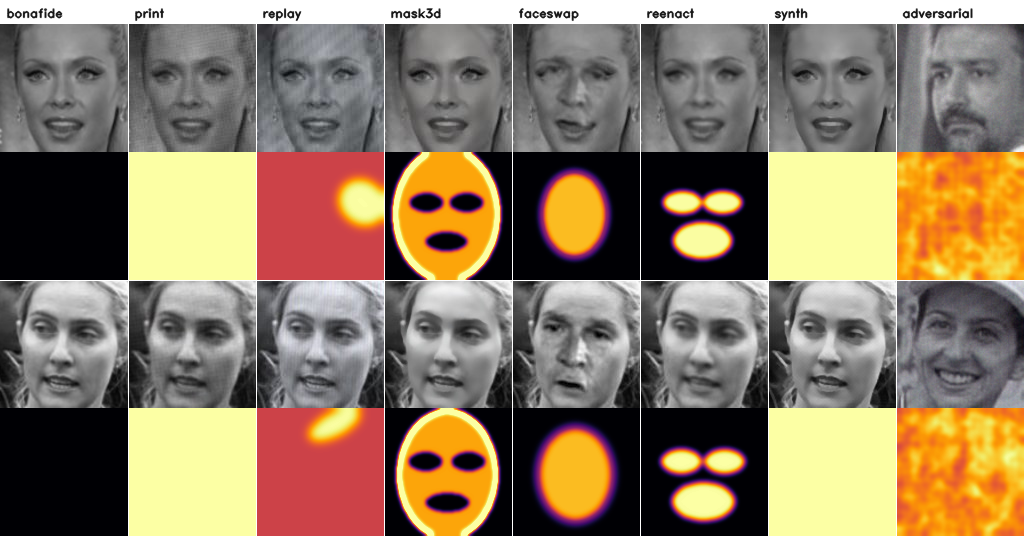
\includegraphics[width=\colw]{figures/taxonomy.png}
\caption{Attack taxonomy and masks}
\label{fig:taxonomy}
\end{figure}

For two source identities the upper strip of Fig.~\ref{fig:taxonomy} shows the eight
classes and the lower strip shows the evidence mask used to train and score the
localiser. Print and replay change the whole capture. 3-D mask, face-swap,
reenactment and adversarial attacks have a local support.

\textbf{Difficulty calibration.} A simulated benchmark is useless if a simple probe can
solve it. The strength $s$ is swept and the largest value is chosen at which a
reference detector (CDCN++) does \emph{not} saturate on the binary or the eight-way
task. This gives $s=0.62$, where the reference detector reaches $1.92\%$ ACER but only
$91.0\%$ eight-way accuracy and $3.74\%$ calibration error, with a worst per-family
APCER of $2.67\%$. The binary task is close to, but not at, the ceiling, while family
discrimination, calibration and unseen attacks remain open. This matches the pattern
reported for UniAttackData \cite{yu2024unified}.

\textbf{Protocols.} In P1 (seen attacks) all eight families appear in train,
validation and test with identity-disjoint splits. In P2 (leave-one-attack-out) one
family is removed from training and appears only at test time. P2 reports ACER, the
detection rate of the held-out family and the \emph{novelty AUROC}, which measures how
well the uncertainty of the model ranks the held-out family above the attack families
seen in training. In P3 (cross-domain) the model is trained on Domain A and tested on
Domain B without any adaptation. All thresholds are fixed at the equal-error point of
the validation split. Following ISO/IEC 30107-3 \cite{iso30107}, APCER is the worst
error over attack families, BPCER is the rate of rejected genuine faces and
\begin{equation}
\mathrm{ACER} = \tfrac{1}{2}\bigl(\mathrm{APCER}+\mathrm{BPCER}\bigr).
\label{eq:acer}
\end{equation}
Eq.~\eqref{eq:acer} is the main error measure in all tables.

\sub{Central-Difference and Spectral Stem}
Central Difference Convolution \cite{yu2020cdcn} mixes a normal convolution with its
local gradient response,
\begin{equation}
y(p_{0}) \;=\; \sum_{p\in\mathcal{N}} w(p)\,x(p_{0}+p)
\;-\;\theta \Bigl(\sum_{p\in\mathcal{N}} w(p)\Bigr) x(p_{0}).
\label{eq:cdc}
\end{equation}
The second term of Eq.~\eqref{eq:cdc} strengthens the part of the response that does
not depend on brightness and costs only one $1\times1$ convolution. Four strided CDC
stages reduce a $112^{2}$ input to $7^{2}$ and pass the $28^{2}$ and $14^{2}$ maps to
the localisation decoder.

Periodic structure such as a display grid or an upsampling checkerboard is lost in a
$7\times7$ token grid. A small spectral branch is therefore added. The log-magnitude
DFT of the brightness channel is pooled onto a polar grid of $16$ radii and $12$
angles, which does not change with translation. A two-layer MLP turns this profile
into four spectral tokens that are added to the spatial tokens. The same profile is
copied into the evidence record so that the peak frequency, its strength and the
direction spread can be quoted in the explanation.

\sub{Adaptive Quantum Attention}
\textbf{Amplitude encoding.} For a head of dimension $d$, queries and keys are scaled
to unit length, $\ket{\psi^{Q}_{i}} = \bs{q}_{i}/\lVert\bs{q}_{i}\rVert$ and
$\ket{\psi^{K}_{j}} = \bs{k}_{j}/\lVert\bs{k}_{j}\rVert$. This is a real amplitude
encoding of $d=2^{n}$ values over $n$ notional qubits.

\textbf{Rotation circuit.} A depth-$L$ circuit acts on a ring of amplitudes. Each layer
rotates disjoint neighbouring pairs, alternating the pairs between layers, with one
learnable angle per rotation,
\begin{equation}
G(\vartheta)=\begin{pmatrix}\cos\vartheta & -\sin\vartheta\\
\sin\vartheta & \cos\vartheta\end{pmatrix},
\qquad
U(\bs{\vartheta})=\prod_{\ell=1}^{L}\ \bigotimes_{k} G(\vartheta_{\ell k}).
\label{eq:givens}
\end{equation}
The circuit in Eq.~\eqref{eq:givens} is the real-valued form of a hardware-efficient
ansatz with nearest-neighbour gates \cite{cherrat2024qvt}. Since $U$ is a product of
rotations it stays exactly orthogonal during training. The measured norm error stayed
below $10^{-6}$, so no extra penalty is needed. It costs only $L\lfloor d/2\rfloor$
angles, which is $\mathcal{O}(dL)$ instead of $\mathcal{O}(d^{2})$
\cite{cherrat2024qvt,evans2025on}. Because it keeps vector length unchanged the score
below is a true probability.

\textbf{Born channel.} Queries and keys are rotated by two \emph{different} circuits,
since a shared circuit would cancel out of the inner product. The score is the
Born-rule transition probability,
\begin{equation}
S_{ij} \;=\; \bigl\lvert \bra{\psi^{Q}_{i}} U_{Q}^{\!\top} U_{K} \ket{\psi^{K}_{j}} \bigr\rvert^{2}
\;\in\;[0,1].
\label{eq:born}
\end{equation}
The score in Eq.~\eqref{eq:born} is quadratic. It does not change when either state
flips sign and it is equally high for alignment or opposite alignment. An interference
pattern has exactly this property, because a moir\'e fringe and its negative carry the
same evidence, whereas a dot product treats them as opposites.

\textbf{Adaptive gating.} Not every kind of evidence is interference-like. A blending
edge, for example, is a plain edge. A gate for each head, computed from simple
statistics of the token set, decides the mix of the two channels,
\begin{align}
\bs{g} &= \sigma\bigl(\bs{W}_{g}\,[\,\mathrm{mean}_t(\bs{X}) \,\Vert\, \mathrm{std}_t(\bs{X})\,] + \bs{b}_{g}\bigr) \in [0,1]^{H_{\text{heads}}},
\label{eq:gatevec}\\
\bs{A} &= \mathrm{softmax}\Bigl( (1-g_{h})\tfrac{\bs{Q}\bs{K}^{\!\top}}{\sqrt{d}} \;+\; g_{h}\,\beta\, \bs{S} \Bigr),
\label{eq:gate}
\end{align}
with $\beta$ a learnable temperature. In Eq.~\eqref{eq:gatevec} $\bs{W}_{g}$ starts at
zero and $\bs{b}_{g}$ at $-2$, so the gate starts near $0.12$. Every block uses
LayerScale \cite{touvron2021cait} with residual gains that start at $10^{-2}$. The
network therefore begins as a plain convolutional model and slowly adds attention,
with the Born channel of Eq.~\eqref{eq:gate} gaining weight only as training goes on.
In tests with an equal budget, removing LayerScale let the new attention add noise to
the stem and slowed training. The final gate value is reported in the explanation,
which makes the mechanism open to inspection.

\textbf{Entropy band.} Let $\mathcal{H}=\mathbb{E}_{t}\bigl[-\sum_{j}A_{ij}\log
A_{ij}\bigr]$ be the mean row entropy of the attention matrix over $T$ tokens. A very
low value means attention has collapsed onto one token. A very high value means it
has spread evenly and carries no information. A two-sided hinge keeps it inside a band,
\begin{equation}
\mathcal{L}_{\text{coh}} = \bigl[\lambda_{\text{lo}}\log T - \mathcal{H}\bigr]_{+}
+ \bigl[\mathcal{H} - \lambda_{\text{hi}}\log T\bigr]_{+},
\label{eq:coh}
\end{equation}
where Eq.~\eqref{eq:coh} uses $(\lambda_{\text{lo}},\lambda_{\text{hi}})=(0.30,0.80)$.

\sub{Quantum Evidence Basis}
Let $\{\ket{e_{b}}\}_{b=1}^{B}$ be the first $B$ standard basis vectors and
$V(\bs{\phi})$ a second rotation circuit of the same kind as Eq.~\eqref{eq:givens}.
The evidence basis is $\ket{\phi_{b}} = V(\bs{\phi})\ket{e_{b}}$, which stays exactly
orthonormal for every $\bs{\phi}$. Measuring the output token states against it gives
the Born probabilities
\begin{equation}
\Pi_{tb} \;=\; \bigl\lvert \braket{\phi_{b}}{\psi_{t}} \bigr\rvert^{2},
\qquad \textstyle\sum_{b}\Pi_{tb}\le 1 .
\label{eq:basis}
\end{equation}
The tensor $\bs{\Pi}$ of Eq.~\eqref{eq:basis} has two jobs. Its average over tokens is
added to the classification features. The same tensor, not an approximation of it, is
exported as the explanation. A small extra classifier trained on
$\overline{\bs{\Pi}}$ with cross-entropy pushes each mode to respond to one class, so
that after training each mode can be \emph{named} after the family it responds to
most (Table~\ref{tab:modes}). These names are read from the trained model and are not
assigned by hand.

\sub{Decoupled Evidential Head}
A Dirichlet distribution is fully described by a direction on the simplex and a
concentration. The standard evidential method \cite{sensoy2018edl} predicts all $K$
concentrations together. Here the two parts are predicted separately,
\begin{align}
\bs{\pi} &= \mathrm{softmax}(\bs{W}_{c}\,\bs{h}), \label{eq:dir}\\
E &= \exp\bigl(\mathrm{clip}(f_{e}(\mathrm{sg}[\bs{z}]))\bigr), \label{eq:mag}
\end{align}
where Eq.~\eqref{eq:dir} gives the class direction, Eq.~\eqref{eq:mag} gives the
amount of evidence and $\mathrm{sg}[\cdot]$ is a stop-gradient. Following subjective
logic \cite{josang2016subjective}, the concentrations, total strength and vacuity are
\begin{equation}
\bs{\alpha} = \bs{1} + E\,\mathrm{sg}[\bs{\pi}], \qquad S = K + E, \qquad
u = \frac{K}{S}.
\label{eq:vacuity}
\end{equation}
From Eq.~\eqref{eq:vacuity} the belief masses are $b_{k}=E\pi_{k}/S$ and the projected
probability under a uniform base rate is $\hat{p}_{k}=(1+E\pi_{k})/(K+E)$. The
direction $\bs{\pi}$ is reported as the belief and $u$ as the uncertainty.

This split has three effects that were checked in tests with equal budgets. First,
$\arg\max_{k}\hat{p}_{k}=\arg\max_{k}\pi_{k}$, so the class decision is trained with
plain cross-entropy. The joint form sends every gradient through $\bs{\alpha}$, where
the usual KL term pushes the pre-activation negative until the gradient vanishes.
This \emph{evidence starvation} was measured directly. Replacing the joint head with
the split head recovered several points of eight-way accuracy. Second, adding
uncertainty cannot reduce detection accuracy, because the magnitude branch only reads
a stop-gradient copy of the shared features. Third, suppressing evidence becomes a
one-dimensional problem. All concentration lives in the single number $E$, so an
out-of-taxonomy constraint cannot bend the class direction.

The evidential loss joins cross-entropy on the direction, a Brier fit on the
concentration \cite{sensoy2018edl} and a term that ties the evidence to correctness,
\begin{equation}
\mathcal{L}_{\text{ev}} = \mathrm{CE}(\bs{\pi},y)
\;+\; \tfrac{1}{2}\,\mathbb{E}\bigl[\lVert \bs{y}-\hat{\bs{p}}\rVert^{2}\bigr]
\;+\; \lambda_{c}\,\mathrm{BCE}\bigl(1-u,\;\mathbb{1}[\hat{y}=y]\bigr),
\label{eq:evloss}
\end{equation}
with $\lambda_{c}=0.4$. The Brier form in Eq.~\eqref{eq:evloss} is used instead of the
digamma-based likelihood because the gradient of the latter almost vanishes while the
Dirichlet is still close to uniform, which is the state of a newly started model.
The usual KL term is dropped. In the split head the wrong-class evidence is already
$E\pi_{k}$, which cross-entropy drives to zero by sharpening $\bs{\pi}$. Keeping the
KL term made short-schedule models saturate at $u\approx1$ everywhere. The
correctness term trains $1-u$ directly as the probability that the decision is right
and makes vacuity useful within about two epochs. In a leave-one-attack-out test this
term moved the AUROC with which vacuity separates a held-out family from genuine
samples from $25.6\%$ (inverted) to $73.9\%$.

\sub{Pseudo-Unseen Evidence Suppression}
A trained stand-in for unknown inputs gives better uncertainty than an internal score
alone \cite{hendrycks2019oe}, but attack detection has no natural pool of outliers.
PUES builds one from the taxonomy itself. Two training images $\bs{x}_{a},\bs{x}_{b}$
from \emph{different} attack families are mixed with $\lambda\sim\mathrm{Beta}(2,2)$
as $\tilde{\bs{x}}=\lambda\bs{x}_{a}+(1-\lambda)\bs{x}_{b}$. No single physical or
generative process can produce such a blend, so it lies outside the taxonomy. Its
evidence is kept well below that of real samples,
\begin{equation}
\mathcal{L}_{\text{PUES}} =
\frac{\bigl[\;\overline{\lVert\tilde{\bs{e}}\rVert_{1}}
      \;-\;\rho\,\overline{\lVert\bs{e}\rVert_{1}}^{\,\text{sg}}\;\bigr]_{+}}
     {\overline{\lVert\bs{e}\rVert_{1}}^{\,\text{sg}}+1},
\qquad \rho = 0.25,
\label{eq:pues}
\end{equation}
where bars in Eq.~\eqref{eq:pues} are batch means. The \emph{relative} form matters.
An absolute target $\lVert\tilde{\bs{e}}\rVert_{1}\to0$ is met trivially by giving
zero evidence everywhere. This failure was seen in an early version, which fell to
$12.5\%$ accuracy over eight classes. Tying the target to the evidence of real samples
in the same batch removes the shortcut. Unlike mixup \cite{zhang2018mixup}, which
asks for a mixed \emph{label}, PUES asks for an \emph{absence of belief}, which is only
possible because the head is evidential.

\sub{Evidence Localisation}
A light feature-pyramid decoder joins the $7^{2}$ token map with the $14^{2}$ and
$28^{2}$ stem maps and predicts $\bs{M}$ at half the input resolution. It is trained
against the ground-truth mask $\bs{M}^{\star}$ of the operator with
\begin{equation}
\mathcal{L}_{\text{loc}} = \mathrm{BCE}(\bs{M},\bs{M}^{\star})
+ \mathrm{Dice}(\bs{M},\bs{M}^{\star}),
\label{eq:loc}
\end{equation}
where the Dice term of Eq.~\eqref{eq:loc} follows \cite{milletari2016vnet}. Unlike
depth supervision \cite{liu2018auxiliary,yu2021revisiting} this target is the actual
support of the evidence and is defined for digital attacks as well as physical ones.

\sub{Risk Calibration}
Attack families are not equally harmful. With severity weights $\bs{\varsigma}$, an
unknown-attack severity $\varsigma_{\text{unk}}$ and evidence area $a=\overline{M}$,
\begin{equation}
r = (1-u)\sum_{k}\hat{p}_{k}\varsigma_{k} \;+\; \lambda_{u}\,u\,\varsigma_{\text{unk}}
\;+\; \lambda_{a}\,a .
\label{eq:risk}
\end{equation}
The first term of Eq.~\eqref{eq:risk} is the expected harm under the posterior,
reduced when evidence is low. The second term adds a premium for unknown attacks, so
an input that is clearly unknown is escalated instead of passed. The third term
rewards evidence that is spread over a clear region. All coefficients and the band
edges that turn $r$ into a Low, Medium, High or Critical label are set as deployment
policy and are not learned, so that an operator can inspect and adjust them. A
vacuity of $u\ge0.55$ sends the sample to a human reviewer.

\sub{Evidence-Grounded Reasoning}
Every forward pass writes a typed evidence record holding the posterior
$\hat{\bs{p}}$, the vacuity $u$, the risk score and band, the top facial regions of
$\bs{M}$ with their mean response, the area and spread of $\bs{M}$, the three
strongest quantum modes with their names and activations, the spectral descriptors
and the mean gate value. Text is generated \emph{only} from this record. The grounded
generator used for all results in this paper is deterministic. Each sentence is
emitted by a rule whose guard is a numeric condition on the record, so every sentence
traces back to a measured value and no fact can be invented. It runs in under a
millisecond with no network call. An optional back-end hands the record to a hosted
multimodal language model with an instruction to paraphrase only, then checks every
number in the result against the record. This reverses the usual setup of language
model forensics \cite{huang2024ffaa,guo2025m2f2det}, in which the language model sees
the image but not the state of the detector.

\sub{Training Objective}
The full loss is
\begin{equation}
\mathcal{L} = \mathcal{L}_{\text{ev}} + w_{m}\mathcal{L}_{\text{loc}}
+ w_{b}\mathcal{L}_{\text{basis}} + w_{s}\mathcal{L}_{\text{sup}}
+ w_{p}\mathcal{L}_{\text{PUES}} + w_{c}\mathcal{L}_{\text{coh}},
\label{eq:total}
\end{equation}
where Eq.~\eqref{eq:total} uses
$(w_{m},w_{b},w_{s},w_{p},w_{c})=(0.6,0.25,0.3,0.15,0.02)$ and combines
Eqs.~\eqref{eq:coh}, \eqref{eq:evloss}, \eqref{eq:pues} and~\eqref{eq:loc}. The term
$\mathcal{L}_{\text{basis}}$ is the cross-entropy of the mode classifier and
$\mathcal{L}_{\text{sup}}$ is a cross-entropy over the three super-classes (genuine,
physical and digital) found by summing $\hat{p}$ within each group. A mix-up between
two families in the same super-class is therefore punished less than one that
crosses the physical and digital boundary.

For the main seen-attack results three more terms act on the predicted distribution
and add no parameters. The classification term is scaled by the focal factor
$(1-\hat{p}_{y})^{\gamma}$ with $\gamma=2$ \cite{lin2017focal}. A binary cross-entropy
$\mathcal{L}_{\text{bin}}$ on the attack probability $1-\hat{p}_{0}$ (weight $0.5$)
protects the attack or genuine decision on which ACER is based. A pair penalty
\begin{equation}
\mathcal{L}_{\text{pair}} = \sum_{(c,c')} w_{cc'}\,
\mathbb{E}_{i\,\mid\,y_i=c}\bigl[\hat{p}_{c'}(x_i)\bigr]
\label{eq:pair}
\end{equation}
reduces the confusions seen during development. In Eq.~\eqref{eq:pair} face-swap with
reenactment and 3-D mask with synthetic are punished in both directions with
$w=0.15$, while replay with print and face-swap with print use $w=0.05$. Each pair is
averaged over its own samples. The baselines get the same focal factor and binary
term together with a pooled pair penalty over the first two pairs with weight $0.15$.

% =====================================================================
\section{Results and Discussion}\label{sec:exp}
% =====================================================================

\sub{Experimental Setup}
Every model is trained from scratch without pretrained weights, so the comparison is
between designs and losses and not between pretraining datasets. Training budgets
differ between protocols, so models are compared only within a table.

For P1 (Table~\ref{tab:main}) X-UAD, CDCN++ and ResNet-18 are trained for $12$ epochs
on the full $19{,}200$-sample training split with the focal factor, binary term and
pair penalty. The kept checkpoint is the epoch with the best validation eight-way
accuracy plus macro-F1 among the epochs whose validation ACER is within $0.5$ points
of the best so far. Seven X-UAD variants were trained under this budget and the one
with the lowest validation ACER is reported. Each baseline was trained once, so X-UAD
received more tuning. ViT-Tiny was not retrained under this recipe. At the original
$10$-epoch budget it stays near chance and its row in Table~\ref{tab:main} comes from
that run.

The other protocols use the original recipe without the three extra terms. P3 reuses
the $10$-epoch P1 checkpoints. P2 and its open-set ablation use $5$ epochs on a fixed
$4{,}800$-sample subset ($4{,}382$ after the held-out family is removed) and the
component ablation uses $5$ epochs on $3{,}592$ samples. All runs use batch size $48$,
AdamW ($\text{lr}=2.5\times10^{-3}$, weight decay $0.02$) with a one-cycle schedule,
gradient clipping at $3.0$ and $112\times112$ random crops from $128$\,px images with
flips and mild brightness changes. Geometric warps are not used because they would
destroy the periodic patterns. Everything runs on CPU with a single seed (0). Models
are compared with McNemar's exact test on paired errors, which says nothing about
variation across seeds.

The first baseline is ResNet-18 \cite{he2016resnet}, a residual CNN of matched
width. The second is ViT-Tiny \cite{dosovitskiy2021vit}, a patch-16 transformer with
normal attention as in the ViT-B/16 entry of \cite{yu2024unified}. The third is CDCN++
\cite{yu2020cdcn,yu2021revisiting}, a central-difference network with pixel-wise map
supervision. CDCN++ shares the stem of X-UAD, so comparing against it shows what the
transformer, the Born channel, the evidential head and the reasoning module add.

\sub{Seen Attacks (P1)}

\begin{table*}
\centering
\caption{Results on P1}
\label{tab:main}
\scriptsize
\begin{tabular}{lcccccccccc}
\toprule
Method & Params & ACER$\downarrow$ & APCER$\downarrow$ & BPCER$\downarrow$ & AUC$\uparrow$ & EER$\downarrow$ & ACC$_8\uparrow$ & F1$_{\text{macro}}\uparrow$ & ECE$\downarrow$ & ECE$_{\text{TS}}\downarrow$ \\
 & (M) & (\%) & (\%) & (\%) & (\%) & (\%) & (\%) & (\%) & (\%) & (\%) \\
\midrule
ResNet-18~\cite{he2016resnet} & 1.59 & 1.88 & 3.08 & 0.67 & 99.95 & 0.67 & \textbf{96.93} & \textbf{96.92} & \textbf{2.35} & \textbf{0.34} \\
ViT-Tiny~\cite{dosovitskiy2021vit}$^{\dagger}$ & 0.64 & 49.75 & 60.67 & 38.83 & 73.43 & 34.65 & 51.27 & 46.04 & 0.67 & -- \\
CDCN++~\cite{yu2020cdcn} & 0.53 & 0.46 & 0.42 & \textbf{0.50} & \textbf{99.99} & \textbf{0.33} & 95.19 & 95.17 & 5.07 & 0.46 \\
\textbf{X-UAD (proposed)} & 1.29 & \textbf{0.42} & \textbf{0.33} & \textbf{0.50} & 99.98 & 0.42 & 94.06 & 94.06 & 5.17 & 0.60 \\
\bottomrule
\end{tabular}
\end{table*}

Table~\ref{tab:main} uses $9{,}600$ identity-disjoint test samples. ACC$_8$ is
eight-way family accuracy and ECE$_{\text{TS}}$ is ECE after temperature scaling
fitted on the validation split. Bold marks the best of the three detectors trained
under the common recipe. ViT-Tiny (marked $^{\dagger}$) uses the original $10$-epoch
recipe and its low ECE reflects a detector near chance.

P1 is close to saturated for every model with a convolutional front end. ResNet-18,
CDCN++ and X-UAD all reach at least $99.95\%$ AUC and at most $1.9\%$ ACER, which
matches the seen-attack results of \cite{yu2024unified}. On the attack or genuine
decision X-UAD has the lowest ACER at $0.42\%$ against $0.46\%$ for CDCN++. The two
models disagree on only $22$ test samples, $10$ in favour of X-UAD and $12$ against
($p=0.83$), so this is a tie. Against ResNet-18 the difference is clear with $74$
discordant samples in favour of X-UAD against $12$ ($p=4.7\times10^{-12}$).
Table~\ref{tab:pertype} lists the APCER of each family, where the ISO APCER is the
worst column. ResNet-18 misses $3.1\%$ of face-swaps, while the worst family of X-UAD
is replay at $0.33\%$.

\begin{table}
\centering
\caption{Per-family APCER (\%)}
\label{tab:pertype}
\scriptsize
\fittab{\begin{tabular}{lcccccccc}
\toprule
Method & Print & Replay & 3D mask & Face-swap & Reenact & Synthetic & Adversarial & Worst \\
\midrule
ResNet-18~\cite{he2016resnet} & 0.33 & 0.33 & 0.00 & 3.08 & 1.33 & 0.75 & 0.00 & 3.08 \\
ViT-Tiny~\cite{dosovitskiy2021vit}$^{\dagger}$ & 40.25 & 0.00 & 4.42 & 60.67 & 60.00 & 59.67 & 0.00 & 60.67 \\
CDCN++~\cite{yu2020cdcn} & 0.08 & 0.00 & 0.00 & 0.42 & 0.17 & 0.00 & 0.00 & 0.42 \\
\textbf{X-UAD (proposed)} & 0.08 & 0.33 & 0.00 & 0.17 & 0.17 & 0.08 & 0.00 & 0.33 \\
\bottomrule
\end{tabular}}
\end{table}

\begin{figure}
\centering
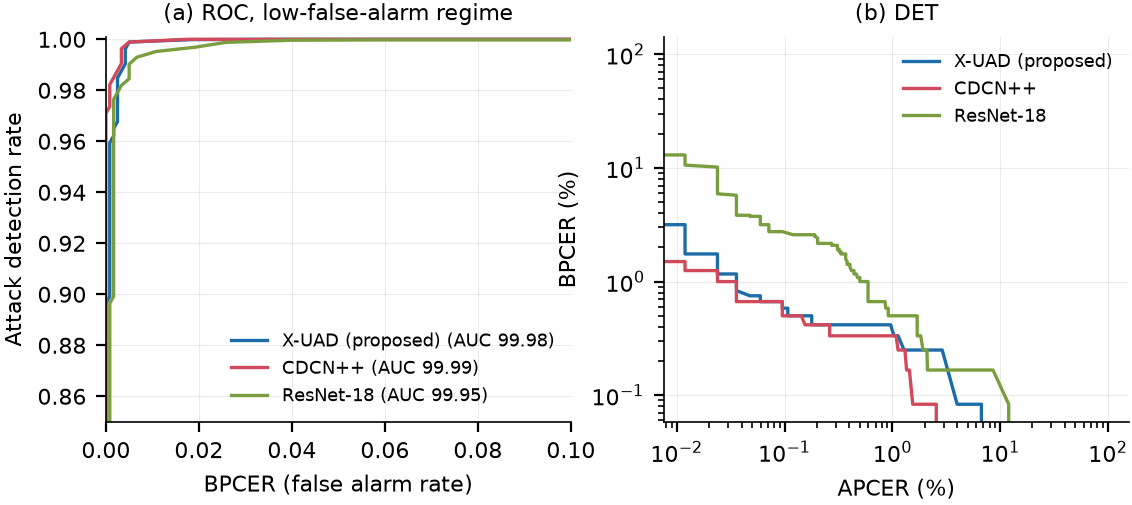
\includegraphics[width=\colw]{figures/roc_det.png}
\caption{ROC and DET curves}
\label{fig:roc}
\end{figure}

The eight-way decision goes the other way. ResNet-18 reaches $96.93\%$ and CDCN++
$95.19\%$ against $94.06\%$ for X-UAD. Both differences are significant ($443$ against
$168$ discordant samples with $p=1.6\times10^{-29}$ and $349$ against $241$ with
$p=1.0\times10^{-5}$). Fig.~\ref{fig:conf} gives the row-normalised confusion matrix
of X-UAD. The largest errors are synthetic predicted as 3-D mask ($7.5\%$), face-swap
and reenactment confused both ways ($5.6\%$ and $5.4\%$) and 3-D mask predicted as
synthetic ($4.6\%$), which are the pairs targeted by Eq.~\eqref{eq:pair}. Two of the
larger errors, synthetic as 3-D mask and face-swap as print ($4.0\%$), cross the
physical and digital boundary. Fig.~\ref{fig:roc} shows the ROC curve in the low false
alarm range together with the DET curve.

\begin{figure}
\centering
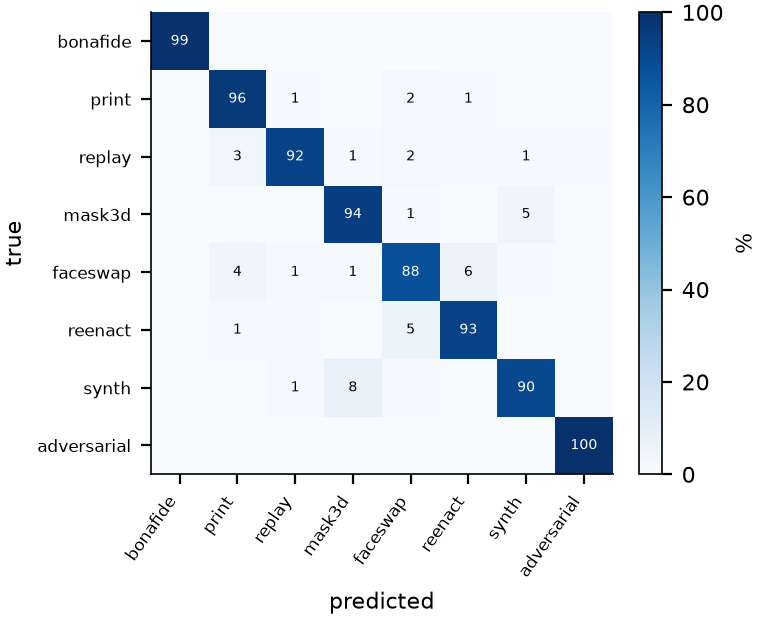
\includegraphics[width=0.82\colw]{figures/confusion.png}
\caption{Confusion matrix of X-UAD}
\label{fig:conf}
\end{figure}

X-UAD shows no calibration advantage for its class posterior. Before correction
ResNet-18 has the lowest ECE ($2.35\%$ against $5.07\%$ for CDCN++ and $5.17\%$ for
X-UAD). After temperature scaling \cite{guo2017calibration} the three reach $0.34\%$,
$0.46\%$ and $0.60\%$ in the same order. What X-UAD adds is a different quantity, the
vacuity of Eq.~\eqref{eq:vacuity}, which is studied as an open-set score in P2. The
plain patch-16 transformer fails at $49.8\%$ ACER. With $16\times16$ patches it never
sees the fine texture of the physical families, which is why X-UAD places a
central-difference stem under its transformer.

\sub{Unseen Attack Families (P2)}
P2 tests what happens when an attack family never seen in training appears at test
time. Table~\ref{tab:loao} holds out one family at a time and reports ACER, eight-way
accuracy, the detection rate of the held-out family and the novelty AUROC. Means are
taken over all four folds and novelty AUROC values below $50$ mean an inverted
ranking.

\begin{table}
\centering
\caption{Results on P2}
\label{tab:loao}
\scriptsize
\fittab{\begin{tabular}{llccccc}
\toprule
Metric & Method & Replay & 3D mask & Face-swap & Adversarial & Mean \\
\midrule
\multirow{3}{*}{ACER (\%)$\downarrow$} & ResNet-18~\cite{he2016resnet} & 51.96 & 30.38 & 49.96 & 30.71 & 40.75 \\
 & CDCN++~\cite{yu2020cdcn} & 25.67 & 39.92 & 25.25 & 25.58 & 29.10 \\
 & \textbf{X-UAD (proposed)} & 26.79 & 21.42 & 38.33 & 39.67 & 31.55 \\
\midrule
\multirow{3}{*}{ACC$_8$ (\%)$\uparrow$} & ResNet-18~\cite{he2016resnet} & 53.94 & 62.66 & 51.39 & 61.53 & 57.38 \\
 & CDCN++~\cite{yu2020cdcn} & 60.62 & 65.07 & 73.23 & 63.84 & 65.69 \\
 & \textbf{X-UAD (proposed)} & 60.95 & 69.01 & 73.34 & 57.59 & 65.22 \\
\midrule
\multirow{3}{*}{Unseen detection rate (\%)$\uparrow$} & ResNet-18~\cite{he2016resnet} & 100.00 & 61.67 & 37.17 & 99.92 & 74.69 \\
 & CDCN++~\cite{yu2020cdcn} & 93.08 & 34.25 & 60.33 & 93.08 & 70.19 \\
 & \textbf{X-UAD (proposed)} & 88.00 & 88.08 & 35.58 & 98.17 & 77.46 \\
\midrule
\multirow{3}{*}{Novelty AUROC (\%)$\uparrow$} & ResNet-18~\cite{he2016resnet} & 35.29 & 56.69 & 74.40 & 36.88 & 50.82 \\
 & CDCN++~\cite{yu2020cdcn} & 49.28 & 66.57 & 81.66 & 55.08 & 63.15 \\
 & \textbf{X-UAD (proposed)} & 71.03 & 50.41 & 87.86 & 43.04 & 63.09 \\
\bottomrule
\end{tabular}}
\end{table}

Mean ACER lies between $29$ and $41\%$ for every method, against under $2\%$ in P1.
This should \emph{not} be read only as the cost of holding out a family, since P2
uses a quarter of the data for half the epochs. The ablation shows the full X-UAD
already at $38\%$ ACER with a similar budget and every family seen
(Table~\ref{tab:abl}). Only comparisons within Table~\ref{tab:loao} are valid. Within
it X-UAD rejects the unseen family most often on average ($77.5\%$ against $74.7\%$
and $70.2\%$, Fig.~\ref{fig:loao}). Its novelty AUROC clearly leads on replay ($71.0$
against $49.3$ and $35.3$) and face-swap ($87.9$ against $81.7$ and $74.4$), trails on
the other two folds and is level with CDCN++ on the mean ($63.09$ against $63.15$).

\begin{figure}
\centering
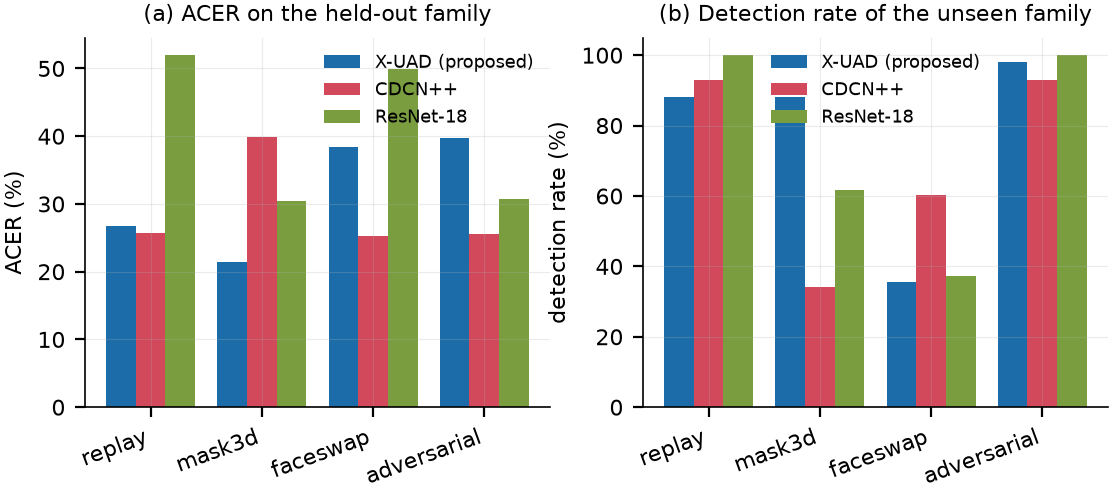
\includegraphics[width=\colw]{figures/loao.png}
\caption{Results on P2 per fold}
\label{fig:loao}
\end{figure}

Panel (a) of Fig.~\ref{fig:loao} shows the ACER of each fold on the full test set and
panel (b) shows the detection rate of the unseen family at the validation threshold.
Rejection and uncertainty ranking are reported separately because they serve
different needs. Rejection matters for operation, while ranking flags that a new
attack type has appeared. The adversarial fold shows the difference. X-UAD rejects
$98.2\%$ of this unseen family while still giving it low vacuity, because the
perturbation sits on top of evidence the model already knows. This fold is also where
the uncertainty is weakest at $43.0$ novelty AUROC.

Scoring the same X-UAD models with their own maximum softmax confidence instead of
vacuity gives $55.9$ mean novelty AUROC against $63.1$ for vacuity. Most of this gain
comes from the replay fold ($71.0$ against $39.5$). It is small on face-swap ($+1.2$)
and adversarial ($+2.3$) and negative on 3-D mask ($-6.4$). On 3-D mask the held-out
family gets the same vacuity as the seen attacks ($0.31$ against $0.32$). On
adversarial it gets \emph{less} ($0.39$ against $0.43$), which explains the inversion.

\sub{Cross-Domain Transfer (P3)}
Domain B differs from Domain A in colour, alignment, resolution and compression all at
once and every method collapses (Table~\ref{tab:cross}). With the source threshold,
BPCER reaches $89$ to $100\%$, so almost every genuine face from the new domain is
rejected. By AUC, CDCN++ keeps the most signal at $65.96$, while ResNet-18 ($46.78$),
ViT-Tiny ($50.18$) and X-UAD ($50.90$) sit at or below chance. The adversarial class is
excluded because it was crafted from Domain A images. This protocol is harsher than
usual cross-dataset tests because four factors change together. None of the proposed
mechanisms targets capture-domain shift, which would need domain generalisation
methods \cite{wang2022ssan,shao2019mada,jia2020ssdg}.

\begin{table}
\centering
\caption{Results on P3}
\label{tab:cross}
\scriptsize
\fittab{\begin{tabular}{lccccc}
\toprule
Method & ACER$\downarrow$ & AUC$\uparrow$ & EER$\downarrow$ & ACC$_8\uparrow$ & ECE$\downarrow$ \\
\midrule
ResNet-18~\cite{he2016resnet} & 49.79 & 46.78 & 51.87 & 2.29 & 83.26 \\
ViT-Tiny~\cite{dosovitskiy2021vit} & 50.00 & 50.18 & 50.23 & 10.31 & 82.47 \\
CDCN++~\cite{yu2020cdcn} & 45.79 & 65.96 & 37.93 & 18.67 & 60.09 \\
\textbf{X-UAD (proposed)} & 49.71 & 50.90 & 49.98 & 3.65 & 81.61 \\
\bottomrule
\end{tabular}}
\end{table}

\sub{Calibration and Localisation}
Fig.~\ref{fig:calib}(a) shows the reliability diagrams before temperature scaling.
All three detectors are somewhat over- or under-confident and temperature scaling
removes most of it for each, so calibration does not separate the models.
Fig.~\ref{fig:calib}(b) shows the uncertainty each model can offer. For the softmax
baselines this is $1-\max_k p_k$. For X-UAD it is the vacuity $u=K/S$, which is
trained as an output in its own right and ranks unseen families above the seen ones
on two of the four folds of Table~\ref{tab:loao}.

\begin{figure}
\centering
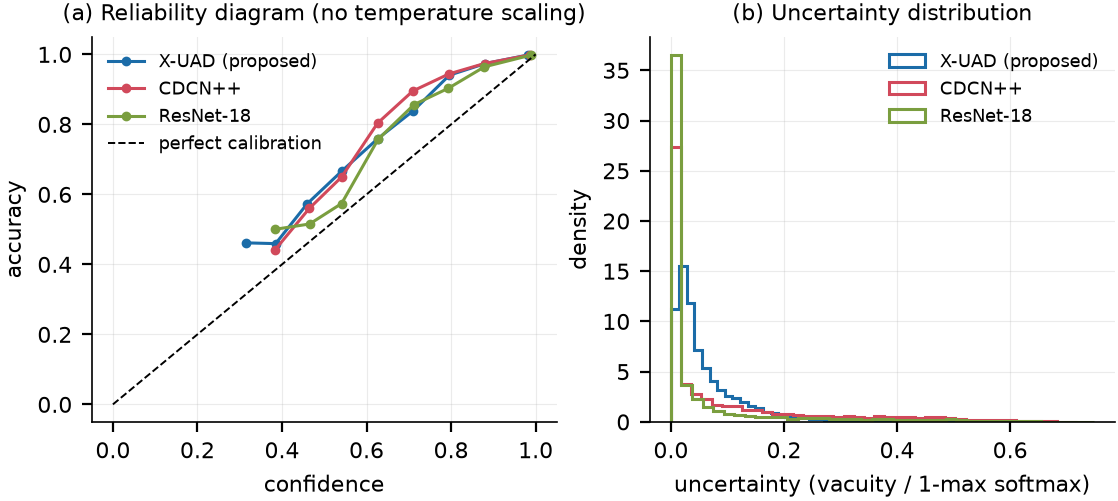
\includegraphics[width=\colw]{figures/calibration.png}
\caption{Calibration and uncertainty}
\label{fig:calib}
\end{figure}

Table~\ref{tab:loc} gives the IoU against the mask of each operator with maps cut at
$0.5$. ResNet-18 and ViT-Tiny give no map. Families whose evidence covers part of the
frame (3-D mask, face-swap and reenactment) are separated from those that change the
whole capture (print, replay and synthetic), since the latter have nearly constant
masks and a trivially high IoU. The region-level mean is the number that shows
whether the localiser works. On all $9{,}600$ test samples X-UAD reaches $80.1\%$
region-level IoU against $73.2\%$ for CDCN++. It is ahead on each of the three
region-level families and on pixel AUC ($97.8\%$ against $96.2\%$, over $40$ samples
per family). Sweeping the cut from $0.10$ to $0.90$ on validation gives a best cut of
$0.55$ for both models, at which the test IoU moves by less than $0.4$ points
($80.1\%$ and $73.5\%$).

\begin{table*}
\centering
\caption{Localisation IoU (\%)}
\label{tab:loc}
\scriptsize
\begin{tabular}{lcccccccc}
\toprule
Method & Print & Replay & 3D mask & Face-swap & Reenact & Synthetic & Region-level mean & Pixel AUC \\
\midrule
CDCN++~\cite{yu2020cdcn} & 96.4 & 93.9 & 76.5 & 75.4 & 67.7 & 97.7 & 73.2 & 96.2 \\
\textbf{X-UAD (proposed)} & 98.1 & 96.9 & 84.2 & 78.8 & 77.2 & 98.2 & 80.1 & 97.8 \\
\bottomrule
\end{tabular}
\end{table*}

\sub{Faithfulness of the Explanation}
An explanation is only useful if changing what it highlights changes the decision.
Table~\ref{tab:faith} gives deletion and insertion AUC \cite{petsiuk2018rise} of the
attack score for the localisation map against a smoothed random field of the same
scale, using $48$ test samples per attack family and $95\%$ bootstrap intervals.
Insertion gain is the map score minus the control score, so an interval below zero
means the map does worse than random.

\begin{table*}
\centering
\caption{Faithfulness of the map}
\label{tab:faith}
\scriptsize
\begin{tabular}{lcccccc}
\toprule
Families & $n$ & \multicolumn{2}{c}{Deletion AUC$\downarrow$} & \multicolumn{2}{c}{Insertion AUC$\uparrow$} & Insertion gain, 95\% CI \\
 & & map & random & map & random & \\
\midrule
Region-level (3D mask, face-swap, reenact) & 144 & 0.892 & 0.941 & 0.935 & 0.942 & [-0.011, -0.003] \\
Whole-frame (print, replay, synthetic, adversarial) & 192 & 0.904 & 0.943 & 0.921 & 0.942 & [-0.026, -0.016] \\
\bottomrule
\end{tabular}
\end{table*}

Deletion is clean. Removing the highlighted pixels lowers the attack score faster
than removing random regions on region-level families ($0.892$ against $0.941$) and
on whole-frame families ($0.904$ against $0.943$). Insertion is not clean. Putting the
highlighted pixels back into a blurred image recovers the score more slowly than
random pixels in both groups. The shortfall is three times larger on whole-frame
families ($-0.021$) than on region-level ones ($-0.007$) but does not vanish. The maps
therefore pass the deletion test and fail the insertion test.

\sub{White-Box Attacks}
The adversarial family of the benchmark is a transfer attack. Here the attacker has
full access to the detector. An $\ell_\infty$ PGD attack \cite{madry2018pgd} ($10$
steps, step size $\varepsilon/4$, random start) is run on $168$ test attacks, $24$
per family. The first goal is evasion, which pushes an attack towards the genuine
class. The second goal targets X-UAD only and lowers $u$ while a cross-entropy term
holds the predicted class fixed. In Table~\ref{tab:whitebox} the upper rows give the
share of attacks still detected and the lower rows give the mean vacuity under the
second attack and how often the predicted class stays the same.

\begin{table*}
\centering
\caption{White-box PGD results}
\label{tab:whitebox}
\scriptsize
\fittab{\begin{tabular}{lccccc}
\toprule
$\varepsilon$ ($\times 1/255$) & clean & 1 & 2 & 4 & 8 \\
\midrule
CDCN++, attacks detected (\%) & 100.0 & 5.4 & 14.9 & 41.1 & 39.3 \\
X-UAD, attacks detected (\%) & 100.0 & 30.4 & 11.3 & 0.0 & 0.0 \\
\midrule
X-UAD, mean vacuity under false-confidence attack & 0.064 & 0.017 & 0.075 & 0.077 & 0.057 \\
X-UAD, predicted class unchanged (\%) & 100.0 & 99.4 & 53.6 & 32.1 & 37.5 \\
\bottomrule
\end{tabular}}
\end{table*}

Neither detector survives evasion. At $\varepsilon=1/255$ X-UAD still catches
$30.4\%$ of the attacks against $5.4\%$ for CDCN++. At $2/255$ both are near $10$ to
$15\%$ and from $4/255$ X-UAD detects none. CDCN++ levels off near $40\%$, which more
likely reflects gradients that are harder to follow than true robustness. None of the
evaded attacks reaches the $u\ge0.55$ referral threshold. The second attack shows that
the uncertainty can be moved on its own. At $\varepsilon=1/255$ it cuts mean vacuity
from $0.064$ to $0.017$ while $99.4\%$ of predicted classes stay the same. At larger
budgets the class is no longer held fixed, so the clean split is a small-perturbation
effect.

\sub{Ablation Study}
Table~\ref{tab:abl} removes one part at a time at a reduced budget. Deltas are
relative to the full model in the first row. These rows are comparable with each
other but not with Table~\ref{tab:main}.

\begin{table*}
\centering
\caption{Component ablation}
\label{tab:abl}
\scriptsize
\begin{tabular}{lcccccc}
\toprule
Variant & ACER$\downarrow$ & AUC$\uparrow$ & ACC$_8\uparrow$ & F1$_{\text{macro}}\uparrow$ & ECE$\downarrow$ & IoU$_{\text{loc}}\uparrow$ \\
\midrule
\textbf{X-UAD (full, reduced budget)} & 38.00 & 87.57 & 69.62 & 69.65 & 2.66 & 64.62 \\
\midrule
\quad w/o Adaptive Quantum Attention & 32.75\,\tiny{(-5.25)} & 91.05\,\tiny{(+3.49)} & 67.45\,\tiny{(-2.18)} & 65.04\,\tiny{(-4.61)} & 3.62\,\tiny{(+0.96)} & 63.36\,\tiny{(-1.26)} \\
\quad w/o evidential head (softmax) & 30.54\,\tiny{(-7.46)} & 91.06\,\tiny{(+3.49)} & 72.07\,\tiny{(+2.45)} & 71.88\,\tiny{(+2.23)} & 3.27\,\tiny{(+0.61)} & 65.02\,\tiny{(+0.41)} \\
\quad w/o spectral branch & 31.13\,\tiny{(-6.87)} & 88.44\,\tiny{(+0.88)} & 70.67\,\tiny{(+1.04)} & 68.92\,\tiny{(-0.73)} & 3.12\,\tiny{(+0.47)} & 64.54\,\tiny{(-0.07)} \\
\quad w/o central-difference stem & 49.08\,\tiny{(+11.08)} & 73.64\,\tiny{(-13.93)} & 48.62\,\tiny{(-21.00)} & 42.16\,\tiny{(-27.49)} & 3.03\,\tiny{(+0.37)} & 52.63\,\tiny{(-11.99)} \\
\quad w/o pseudo-unseen suppression & 26.04\,\tiny{(-11.96)} & 91.08\,\tiny{(+3.51)} & 72.90\,\tiny{(+3.27)} & 72.85\,\tiny{(+3.20)} & 2.83\,\tiny{(+0.17)} & 64.23\,\tiny{(-0.39)} \\
\quad w/o localisation supervision & 33.58\,\tiny{(-4.42)} & 89.17\,\tiny{(+1.61)} & 70.56\,\tiny{(+0.94)} & 68.78\,\tiny{(-0.87)} & 2.41\,\tiny{(-0.25)} & 34.34\,\tiny{(-30.27)} \\
\bottomrule
\end{tabular}
\end{table*}

The central-difference stem matters most. Removing it costs more than all other parts
together, dropping eight-way accuracy by $21$ points and region-level IoU by $12$.
Localisation supervision gives the map its meaning. Without it region-level IoU falls
by more than half while detection barely changes, so a saliency map taken for free
from a detector is not the same as a supervised evidence map.

Two parts trade closed-set accuracy for uncertainty. Removing PUES \emph{improves}
reduced-budget ACER but removes the ability the term was built for.
Table~\ref{tab:oablate} isolates this trade on the face-swap fold, where PUES is worth
$5.4$ novelty AUROC points and $5.2$ points of family accuracy at a cost of $2.2$ ACER
points. AQA shows the same pattern. At reduced budget it costs ACER but improves
calibration and localisation. On the face-swap fold it adds $1.9$ AUC and $1.9$
accuracy at equal novelty AUROC.

\begin{table*}
\centering
\caption{Open-set ablation}
\label{tab:oablate}
\scriptsize
\begin{tabular}{lcccccc}
\toprule
Variant & ACER$\downarrow$ & AUC$\uparrow$ & ACC$_8\uparrow$ & ECE$\downarrow$ & Unseen detect.$\uparrow$ & Novelty AUROC$\uparrow$ \\
\midrule
Full X-UAD & 38.33 & 91.41 & 73.34 & 6.26 & 35.58 & 87.86 \\
w/o pseudo-unseen suppression & 36.17 & 86.33 & 68.12 & 6.78 & 45.50 & 82.43 \\
w/o Adaptive Quantum Attention & 39.83 & 89.47 & 71.40 & 7.36 & 32.75 & 87.89 \\
\bottomrule
\end{tabular}
\end{table*}

\sub{Efficiency and Gate Analysis}
X-UAD adds its extra abilities at a small parameter cost (Table~\ref{tab:eff},
measured on CPU for one $112\times112$ crop). Each rotation circuit costs
$L\lfloor d/2\rfloor$ angles against $d^{2}$ for a dense projection and the reasoning
module runs in under a millisecond with no learned parameters. At $1.29$M parameters
X-UAD sits between ViT-Tiny and ResNet-18 in size while being the only model that
gives a localisation map, named evidence modes and a written explanation. GMAC counts
leave out attention products, so the X-UAD figure is slightly low.

\begin{table*}
\centering
\caption{Inference cost}
\label{tab:eff}
\scriptsize
\fittab{\begin{tabular}{lcccc}
\toprule
Method & Params (M) & GMACs & Latency (ms) & Explanation outputs \\
\midrule
ResNet-18~\cite{he2016resnet} & 1.59 & 0.368 & 16.8 & none \\
ViT-Tiny~\cite{dosovitskiy2021vit} & 0.64 & 0.031 & 2.9 & attention only \\
CDCN++~\cite{yu2020cdcn} & 0.53 & 0.070 & 13.1 & depth-proxy map \\
\textbf{X-UAD (proposed)} & 1.29 & 0.119 & 16.9 & map + modes + text \\
\bottomrule
\end{tabular}}
\end{table*}

Table~\ref{tab:gates} gives the final gate $g$ of Eq.~\eqref{eq:gate}, the share of
the attention score taken from the Born channel, averaged over heads, layers and test
samples of each family. The gate opens widest on print ($0.434$) and adversarial
($0.394$) and least on replay ($0.231$). Replay was expected to be the clearest
interference family because of its moir\'e beat, so the channel is used (mean near
$0.31$) but the reason why it helps is not yet settled.

\begin{table*}
\centering
\caption{Born-channel gate per family}
\label{tab:gates}
\scriptsize
\begin{tabular}{lcccccccc}
\toprule
Attack family & Bonafide & Print & Replay & 3D mask & Face-swap & Reenact & Synthetic & Adversarial \\
\midrule
Mean Born-channel gate $g$ & 0.309 & 0.434 & 0.231 & 0.287 & 0.267 & 0.267 & 0.284 & 0.394 \\
\bottomrule
\end{tabular}
\end{table*}

\sub{Qualitative Results}
The rows of Fig.~\ref{fig:qual} show, for one sample per family, the input, the
predicted evidence map, the ground-truth mask and the AQA attention rollout. The
localiser recovers the eye and mouth support of the reenactment and the holes of the
3-D mask and spreads over the whole frame for print, synthetic and adversarial. It is
not perfect. On this face-swap it predicts an eye and mouth pattern like reenactment
instead of the blending ellipse and on replay it misses the local glare spot.
Table~\ref{tab:modes} lists the quantum evidence modes. Each mode is named after the
family for which its Born activation of Eq.~\eqref{eq:basis} is most selective
($z$-scored across families). These analyses and the gate values use the $10$-epoch
P1 model.

\begin{figure*}
\centering
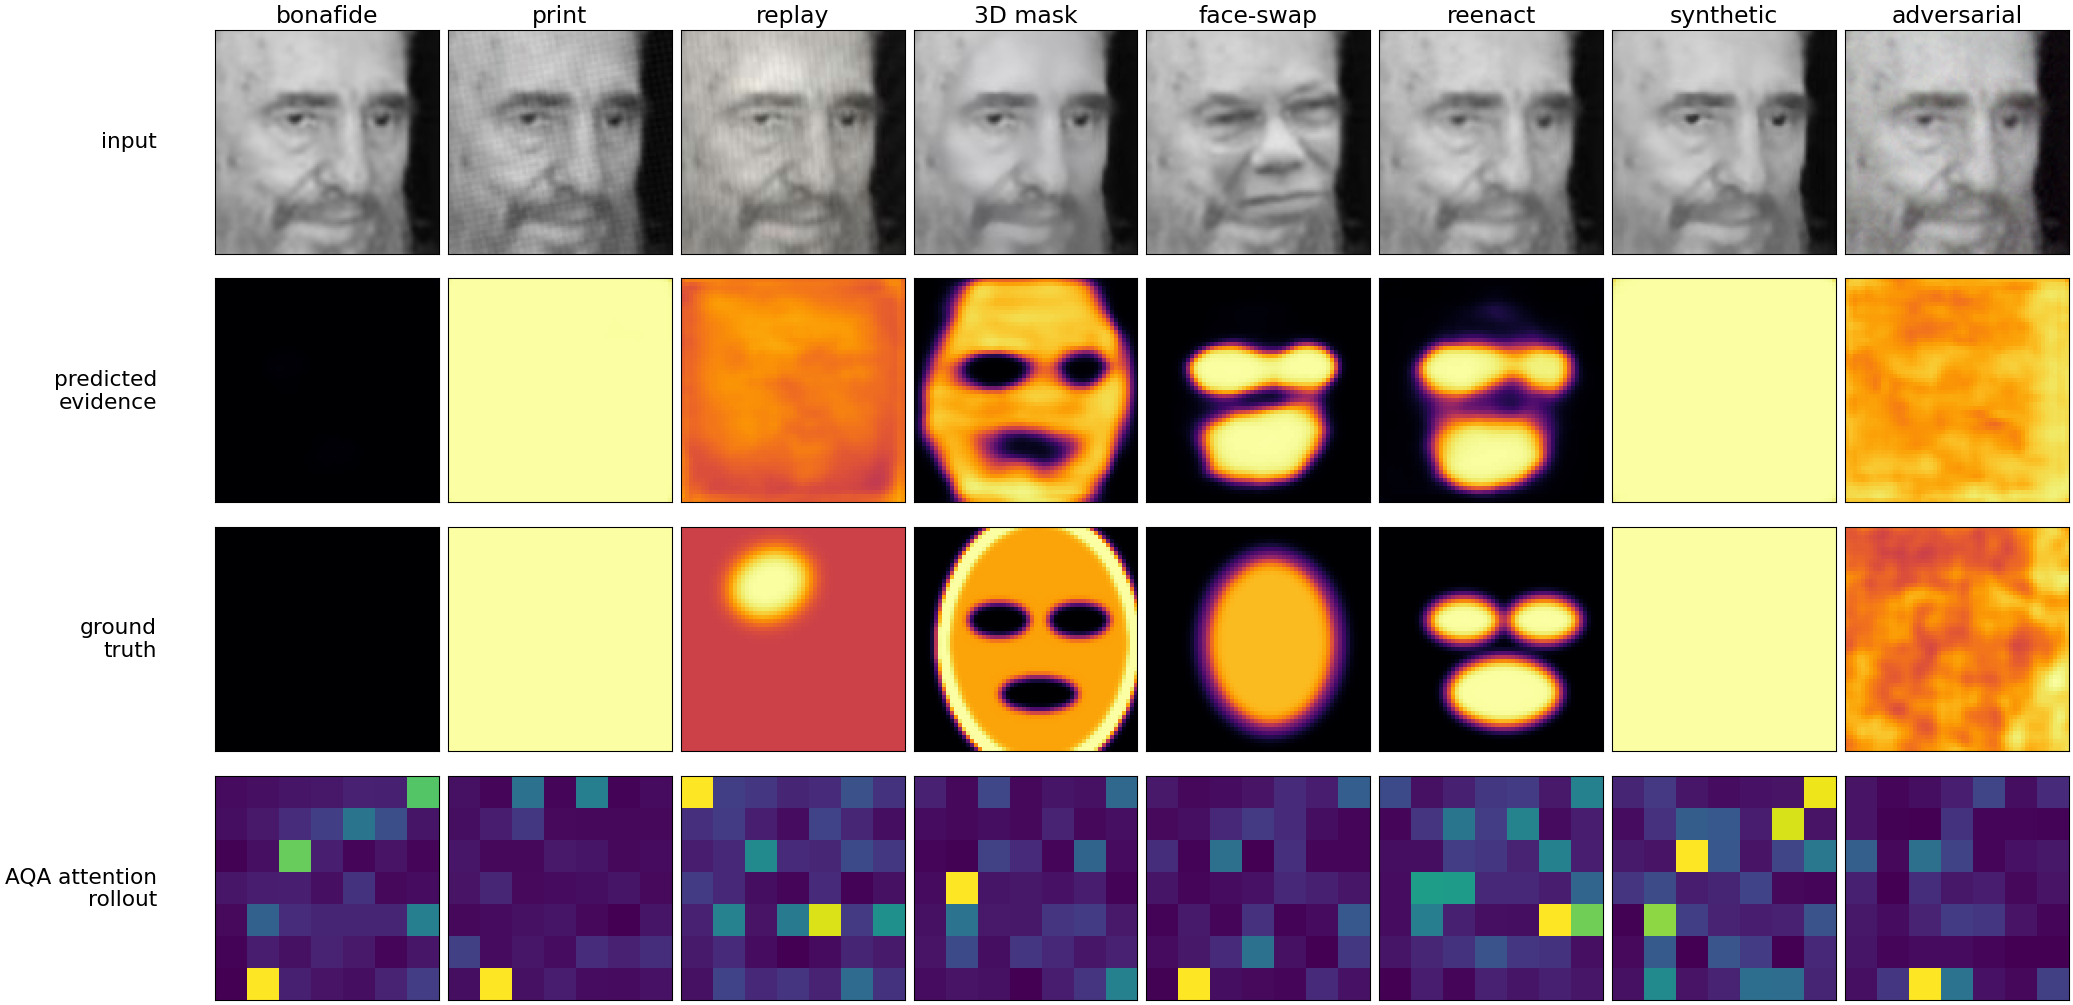
\includegraphics[width=0.62\textwidth]{figures/qualitative.png}
\caption{Qualitative results}
\label{fig:qual}
\end{figure*}

\begin{table*}
\centering
\caption{Learned evidence modes}
\label{tab:modes}
\scriptsize
\fittab{\begin{tabular}{ccccc}
\toprule
Mode & Most selective for & Selectivity ($z$) & Mean activation & Spatial dispersion \\
\midrule
1 & Replay & 2.59 & 0.069 & 0.793 \\
7 & 3D mask & 2.51 & 0.051 & 0.810 \\
3 & Bonafide & 2.45 & 0.058 & 0.835 \\
6 & Adversarial & 2.36 & 0.057 & 0.869 \\
4 & Print & 2.28 & 0.049 & 0.803 \\
5 & Synthetic & 2.01 & 0.043 & 0.767 \\
0 & Reenact & 1.85 & 0.047 & 0.783 \\
2 & Replay & 1.84 & 0.039 & 0.845 \\
\bottomrule
\end{tabular}}
\end{table*}

% =====================================================================
\section{Conclusion}\label{sec:concl}
% =====================================================================
This paper presented X-UAD, a single model that detects physical and digital face
attacks, reports how uncertain it is, marks where the evidence lies and explains its
decision in text that can be checked sentence by sentence. A Born-rule attention
channel matches the interference nature of attack evidence at a cost of
$\mathcal{O}(dL)$ parameters. An orthonormal quantum evidence basis serves both as a
classification feature and as the explanation. Pseudo-unseen evidence suppression
builds an outlier stand-in from the attack taxonomy and turns Dirichlet vacuity into a
usable open-set score. On seen attacks X-UAD matches the strongest baseline on the
attack or genuine decision and localises evidence better than every compared model.
On unseen attack families it gives the highest average detection rate.

The work also has limitations. All numbers come from a single seed on a simulated
benchmark and the adapters for seven public datasets have not yet been run on real
captured data. X-UAD received more tuning than the baselines and the P2, P3 and
ablation tables come from an earlier code version. Eight-way accuracy is lower than
both convolutional baselines and there is no calibration advantage after temperature
scaling. The uncertainty ranking is mildly inverted on the adversarial fold, the
localisation map fails the insertion test, a white-box attacker can switch off the
uncertainty and no method performs acceptably across capture domains. In future work
these limits will be addressed by repeating all experiments over several seeds,
running the released adapters on real captured datasets and giving the baselines the
same tuning budget. Domain generalisation methods will be added to handle camera
shift together with unseen attacks. Adversarial training on the vacuity output and
input consistency checks will be explored to protect the uncertainty. Higher-order
PUES blends will also be tested to improve the outlier stand-in. The referral threshold
will be set from measured referral rates for each group.

\FloatBarrier
\section*{Author Contributions}
Amrutha Babu, Swethaa Premnath and Vividha Senthil Mohan contributed equally to the
conceptualisation, methodology, software, construction of the benchmark,
experiments, formal analysis, visualisation and writing of the original draft.
Muthunagai S U guided the project administration and the editing of the manuscript
and supervised the experimental process. Nivedha K provided critical review and
technical validation. All authors read and approved the final manuscript.

\section*{Acknowledgment}
The authors would like to express their gratitude to their supervisor, Prof.
Muthunagai S U, for her invaluable mentorship, insightful guidance and support
throughout the research. The authors would also like to extend their thanks to the
School of Computer Science and Engineering (SCOPE) at Vellore Institute of Technology
(VIT), Vellore, for its support and for providing the academic resources and
facilities used in this work. This work would not have been possible without the
foundational contributions of the researchers who developed and shared the Labeled
Faces in the Wild (LFW) database \cite{huang2007lfw}, whose work has been
instrumental for the broader research community.

\section*{Data Availability}
The genuine faces of Domain A are taken from the Labeled Faces in the Wild (LFW)
database \cite{huang2007lfw}, a public academic benchmark of $13{,}233$ face
photographs collected from the web. Of these, $12{,}794$ identity-labelled images of
$5{,}616$ subjects were used. LFW is publicly available to the research community at
\url{http://vis-www.cs.umass.edu/lfw/} \cite{lfwweb}. All attack samples were
generated from these images by the benchmark operators of
Section~\ref{sec:method}, so no attack data was collected from people. Domain B
(Wild-Sim) consists of $700$ in-the-wild colour face crops \cite{wildsim} and is used
only for testing. No new images of people were captured, no private data were
collected and no attempt was made to identify any person in the images. The
Wild-Sim face set, the benchmark generator, the dataset configuration files and the
code are available from the corresponding author on reasonable request.

\section*{Funding}
Authors have not received any fund to carry out this research work.

\bibliographystyle{IEEEtran}
\bibliography{refs}

\end{document}
